\section*{Models and Event Log}
The tutorial will use example files that are provided with the tool, which are the event log coded in XES format (log.xes), process model modelled as a Petri Net (model.pnml) and stochastic process model as an SDFA coded in JSON format (automaton.json). Table 1, Figure 1 and Figure 2 represent the three files, respectively. 


\begin{figure}[h!]
\hspace{3mm}
 \begin{minipage}{0.45\textwidth}
\begin{center}
\vspace{-3mm}
\begin{tikzpicture}[scale=0.6, transform shape, ->, >=stealth', shorten >=1pt, auto, node distance=20mm, on grid, semithick, transition/.style={fill=rebeccapurple!30, draw, minimum size=9mm, drop shadow}, place/.style={fill=black!5, draw, circle, minimum size=9mm, drop shadow}]

\node[place,label=90:\small $p_0$]				(p0) 											{\Large $\bullet$};
\node[transition,label=90:\small $t_0$]		(t0) [right=of p0] 				{\Large $\texttt{a}$};
\node[place,label=90:\small $p1$] 				(p1) [above right=of t0]	{};
\node[place,label=270:\small $p_2$] 			(p2) [below right=of t0]	{};
\node[transition,label=90:\small $t_1$] 	(t1) [right=of p1]				{\Large $\texttt{b}$};
\node[transition,label=270:\small $t_3$] 	(t3) [right=of p2]				{\Large $\texttt{c}$};
\node[transition,label=0:\small $t_2$] 		(t2) [below right=of p1,xshift=17pt]				{\Large $\texttt{d}$};
\node[place,label=90:\small $p3$] 				(p3) [right=of t1]				{};
\node[place,label=270:\small $p4$] 				(p4) [right=of t3]				{};
\node[transition,label=90:\small $t_4$] 	(t4) [below right=of p3]	{\Large $\texttt{e}$};
\node[place,label=90:\small $p5$] 				(p5) [right=of t4]				{};

\path (p0) edge node {} (t0)
			(t0) edge node {} (p1)
					 edge node {} (p2)
			(p1) edge node {} (t1)
			(p2) edge node {} (t3)
			(t1) edge node {} (p3)
			(t3) edge node {} (p4)
			(t2) edge node {} (p1)
					 edge node {} (p2)
			(p3) edge node {} (t2)
					 edge node {} (t4)
			(p4) edge node {} (t2)
					 edge node {} (t4)
			(t4) edge node {} (p5)
;
\end{tikzpicture}
\vspace{-2mm}
\caption{Process Model.}
\label{fig:petri:net}
\vspace{-2mm}
\end{center}
\end{minipage}
\hspace{7mm}
\begin{minipage}{0.45\textwidth}
\begin{center}
\vspace{-9mm}
\begin{tikzpicture}[scale=0.65, transform shape, ->, >=stealth', shorten >=1pt, auto, initial text=, node distance=20mm, on grid, semithick, every state/.style={fill=rebeccapurple!30, draw, circular drop shadow, text=black, minimum size=9mm}]
\node[initial,state,label=270:$s_0$]	(s0) 											{$0$};
\node[state,label=270:$s_1$]					(s1) [right=of s0] 				{$0$};
\node[state,label=0:$s_2$]						(s2) [above right=of s1]	{$0$};
\node[state,label=270:$s_3$] 					(s3) [below right=of s2]	{$0$};
\node[state,label=0:$s_4$] 					  (s4) [below right=of s1]	{$\nicefrac{1}{5}$};
\node[state,label=270:$s_5$] 				  (s5) [right=of s3]				{$1$};

\path (s0) edge node {$\texttt{a}(1)$} (s1)
			(s1) edge node {$\texttt{b}(\nicefrac{1}{2})$} (s2)
			     edge node[below, xshift=-14pt, yshift=-2pt] {$\texttt{c}(\nicefrac{1}{2})$} (s4)
			(s2) edge node {$\texttt{c}(1)$} (s3)
			(s3) edge node[above]  {$\texttt{d}(\nicefrac{1}{2})$} (s1)
					 edge node {$\texttt{e}(\nicefrac{1}{2})$} (s5)
			(s4) edge node[below, xshift=16pt, yshift=-2pt] {$\texttt{b}(\nicefrac{4}{5})$} (s3);
\end{tikzpicture}
\vspace{3.5mm}
\caption{Stochastic Process Model.}
\label{fig:SDFA}
\vspace{-10mm}
\end{center}
\end{minipage}

\begin{center}
\vspace{5mm}
\begin{minipage}{0.45\textwidth}
 \centering
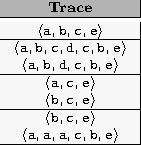
\includegraphics[width=0.40\textwidth]{fig/eventLog.pdf} 
\caption*{ Table 1: Event Log}
\label{fig:Log}
\end{minipage}
\end{center}
\vspace{-4mm}
\end{figure}

All files are located in the folder \textbf{jbpt-pm\slash guide\slash examples}. If the folder does not contain the files, you can download them from \url{https://github.com/jbpt/codebase/tree/master/jbpt-pm/entropia/guide/}. It is recommended to use the event log and models provided to understand how to run the Entropia commands. Then, try it with your own data. Refer to Table III in the demo paper for more details about file types and formats supported by the tool.
